\documentclass[a4paper]{article}
\usepackage[T1]{fontenc}
\usepackage[utf8]{inputenc}
\usepackage[italian]{babel}
\usepackage{enumitem}
\usepackage{graphicx}
\graphicspath{{./images/}}
%\usepackage{geometry} 
%\geometry{a4paper,top=3cm,bottom=3cm,left=3.5cm,right=3.5cm,% heightrounded,bindingoffset=5mm}

\begin{document}

\author{Manuel Trivilino, Davide Salaorni, Luca Terracciano}

\title{\Large Data4Help\\
\Large RASD Requirements Analysis and Specification Document
}

\maketitle
\newpage

\tableofcontents
\newpage

\section{Introduction}

\subsection{Purpose}

\subsection{Scope}

\paragraph{Description of the given problem}

\paragraph{}
TrackMe is a company that develops software-based services for third parties and for consumers. The main service is called Data4Help.
 Data4Help is a service that allows third parties to monitor the location and the health status of individual, it handles a policy of permissions for each user and collects individual’s data from their personal devices.
The service supports the registration of individuals who, by registering, agree that TrackMe acquires their data. After registration, these third parties can request:

\begin{itemize}
    \item Access to the data of some specific individuals (we can assume, for instance, that they know an 
    individual by his/her social security number or fiscal code in Italy). In this case, TrackMe passes 
    the request to the specific individuals who can accept or refuse it.
    
    \item Access to anonymized data of groups of individuals (for instance, all those living in a certain 
    geographical area, all those of a specific age range, etc.). These requests are handled directly 
    by TrackMe that approves them if it is able to properly anonymize the requested data. For 
    instance, if the third party is asking for data about 10-year-old children living in a certain street 
    in Milano and the number of these children is two, then the third party could be able to derive 
    their identity simply having people monitoring the residents of the street between 8.00 and 
    9.00 when kids go to school. Then, to avoid this risk and the possibility of a misuse of data,
    TrackMe will not accept the request. For simplicity, we assume that TrackMe will accept any 
    request for which the number of individuals whose data satisfy the request is higher than 
    1000.

\end{itemize}

\paragraph{}
As soon as a request for data is approved, TrackMe makes the previously saved data available to the 
third party. Also, it allows the third party to subscribe to new data and to receive them as soon as 
they are produced.
TrackMe develops itself two third-party services: AutomatedSOS and Track4Run.

\paragraph{Goals}

\setlist[enumerate]{label*=G.\arabic*}

\begin{enumerate}
	
	%Data4Help
	
	\item Allow users to register in two different ways: single person and third parties.
	\item Third parties can request for users' data.
	    
	    \begin{enumerate}[label*=.\arabic*]
	        \item Third parties can request for anonymized data.
	        \item Third parties can request for a specific person's data.
	    \end{enumerate}
	    
	%AutomatedSOS
	\item The user can receive medical support in case of health emergency thanks to AutomatedSOS.
	
	%Track4Run
	\item Users can organize a run and define its path.
	\item Users can enroll to a run.
	\item Users can be spectators of a run seeing the partecipants' position on a map.
	
\end{enumerate}

\subsection{Definitions, Acronyms, Abbreviation}


\subsection{Revision History}

\subsection{Reference Documents}

\subsection{Document Structure}

\section{Overall Description}

\subsection{Product Perspective}

\begin{figure}[h!]
    \centering
    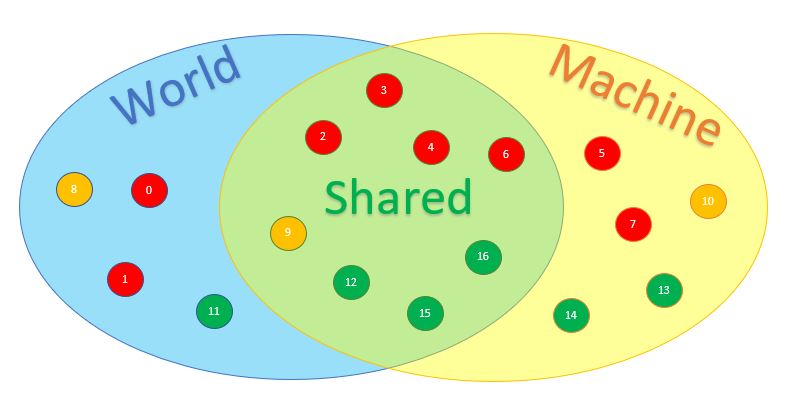
\includegraphics[width=\linewidth]{phenomenaSets}
    \caption{World, machine and shared phenomena.}
    \label{fig:my_label}
\end{figure}

\begin{figure}[h!]
    \centering
    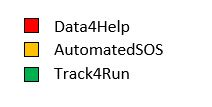
\includegraphics{setsLegend}
    \caption{Legend of the colored circles.}
    \label{fig:my_label}
\end{figure}


\subsection{Product Functions}

\subsection{User Characteristics}

\paragraph{}The following actors are the users of the services offered by TrackMe. 


\begin{itemize}
    \item User:  a person that is successfully registered to TrackMe as consumer and allow to acquire anonymous data, eventually a client of third party services (i.e. AutomatedSOS, Track4Run) that allows even personal data.
    
    \item Third Parties:  a company or a person who is registred to TrackMe as "Third party" that access to anonymous and can require to access to individual data.
    
\end{itemize}

\subsection{Assumption, Dependencies and Constraints}

\subsubsection{Domain Assumptions}


\begin{enumerate}[label={[D.\arabic*]}]
    
    
    \item Registered people log in with his own account, collected data belongs to the account owner and the personal informations (Age, address, sex...) given from the users are correct.
    \item Users log in with devices from which is possible to collect information and data (like smartphones, smartwatches, laptops with an internet connection, sensors like GPS, accelerometer, pulse sensor...).
    \item The data collected from the devices (position and health status) are reliable, accurate and in real time.
    
\end{enumerate}


\section{Specific Requirements}

\subsection{External Interface Requirements}

\subsubsection{User Interfaces}

\subsubsection{Hardware Interfaces}

\subsubsection{Software Interfaces}

\subsubsection{Communication Interfaces}

\subsection{Functional Requirements}

\subsection{Performance Requirements}

\subsection{Design Constraints}

\subsubsection{Standards Compliance}

\subsubsection{Hardware Limitations}

\subsubsection{Any other Constraint}

\subsection{Software System Attributes}

\subsubsection{Reliability}

\subsubsection{Availability}

\subsubsection{Security}

\subsubsection{Maintainability}

\subsubsection{Portability}

\section{Formal Analysis Using Alloy}

\section{Effort Spent}

\section{References}


\end{document}